\documentclass{article}

% Language setting
% Replace `english' with e.g. `spanish' to change the document language
\usepackage[english]{babel}

% Set page size and margins
% Replace `letterpaper' with`a4paper' for UK/EU standard size
\usepackage[letterpaper,top=2cm,bottom=2cm,left=3cm,right=3cm,marginparwidth=1.75cm]{geometry}

% Useful packages
\usepackage{amsmath}
\usepackage{graphicx}
\usepackage[colorlinks=true, allcolors=blue]{hyperref}

\title{Bel e Decibel}
\author{Leonardo Paz Faria}
\date{May 30, 2022}

\begin{document}
\maketitle



\section{Introdução}

O Bel foi criado a partir de estudos feitos por [Alexander Graham Bell(1847 – 1922)] que também foi inventor do telefone. Nesse estudo ele percebeu que a variação de som que o ouvido humano pode sentir não acompanha um a escala linear, onde essa escala é logaritma. Para entender a escala decibel (dB) é importante entendermos sua história para explicar porque ela se tornou tão importante. Ela nasce com a necessidade de especialistas da empresa Bell Labs em definir uma medida de diferença entre dois sinais de potência elétrica (P1 e P2). A motivação de Alexamder foi fazer com que a amplitude do sinal, não se perdesse, fazendo com que o sinal chegasse até o outro lado, indo do ponto A ao B utilizando correção da amplitude do sinal.
\section{Bel}

\subsection{História}

Graham Bell notou que a escala que o ouvido percebe é logaritma. Portanto, ao invés de utilizar a escala linear para representar a amplificação (ganho) ou a atenuação (perda) de um sistema, Graham Bell resolveu utilizar uma escala logaritma. O Sinalenviado por um par de fios esticados entre uma cidade e outra, sofria uma grande atenuação (diminuição na amplitude do sinal).Caso estas perdas não fossem corrigidas por meio de amplificadores, o sinal não chegaria inteligível na outra ponta da transmissão.Graham Bell criou uma unidade de medida para esta atenuação. Esta unidade era chamada originalmente de TU (transmission unit). Mas em 1929, após a sua morte, os engenheiros do Bell Telephone Laboratory resolveram homenagear seu fundador, dando o nome de Bel (símbolo B) a esta unidade de medida.

\begin{figure}[h!]
\centering
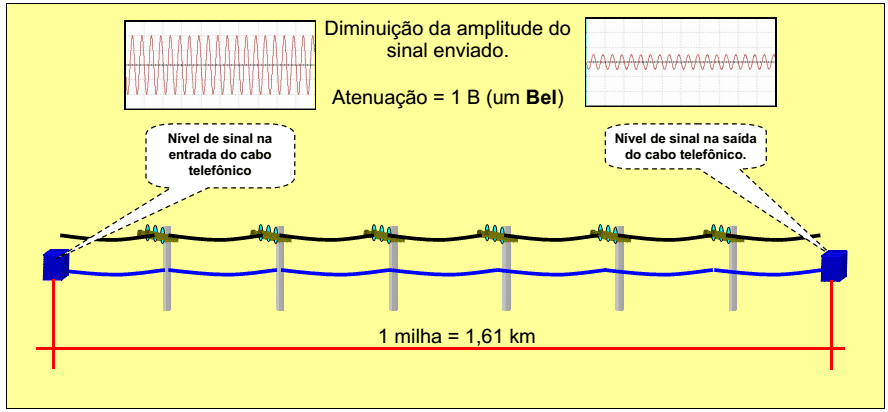
\includegraphics[width=15cm]{Belimagem.png}
\label{fig:Belimagem}
\end{figure}



\subsection{Uso e Formulas}

Com o passar do tempo junto a prática notou-se que 1Bel era muito grande e resultava em números ainda maiores, foi decidido adotar como padrão o Decibel ou seja 1 décimo de Bel.

$$\frac{1B}{10} = 1dB => 10dB = 1B$$

Caso precisemos encontrar um ganho ou aumento na Amplitude do sinal de onda há uma regr a, onde o valor resultante seja positivo significa que há um ganho no sistema, pois o sinal de saída é maior que o de entrada, caso o valor resultante seja negativo significa que há uma perda no sistema:

\begin{center}
 $$\log \frac {(Psaída)}{(Pentrada)} = Ganho(B)$$
\end{center}

Caso queira a relação em Decibel:

\begin{center}
 $$10 . \log \frac {(Psaída)}{(Pentrada)} = Ganho(dB)$$
\end{center}

\begin{figure}[h!]
\centering
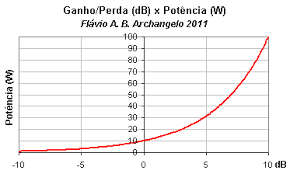
\includegraphics[width=10cm] {grafico.png}
\label{fig:grafico}
\end{figure}


\subsection{Aplicações de decibel na Eletrônica}

Um simples amplificador para um MP3 player já pode dar dor de cabeça suficiente se não for feito uso das ferramentas matemáticas adequadas. Vamos imaginar a seguinte situação: você tem um MP3 player cuja potência máxima de saída é de 20 mW. Nele você quer conectar uma pequena caixa amplificada, cuja potência nominal de saída é de 10 W. Se tínhamos um valor pequeno de potência (os 20 mW do seu MP3 player) e queremos aumentar esta potência (para os 10 W da caixa amplificada), podemos dizer que tivemos um ganho de potência.

\begin{figure}[h!]
\centering
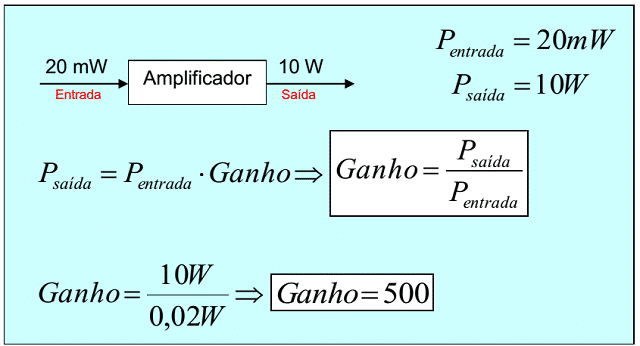
\includegraphics[width=12cm]{formula.png}
\label{fig:formula}
\end{figure}


Como visto na imagem houve um ganho de 500 vezes referente a entrada do sinal.



\section{Conclusão}

É importante perceber que o Decibel é uma ferramenta matemática, cuja função é facilitar os cálculos de circuitos e sistemas eletrônicos. Para não trabalharmos com números muito grandes ou muito pequenos, a conversão para a escala logaritma permite uma melhor percepção dos valores envolvidos, e claramente tem sua participação em aprelhos eletronicos e circuitos onde seus calculos tem de ser minusiosamente bem calculados.

\bibliographystyle{alpha}
\bibliography{sample}

\textbf{Ondas, Acústica, Unidades do Sistema SI e Glossário de Física} Disponível em:
<http://www.feiradeciencias.com.br>. Acesso em 10 de junho de 2021.

NEIVA, Álvaro. Tutorial Sobre Decibéis. Disponível em: <http://geocities.yahoo.com.br/
alvaroneiva/tutdb.htm>. Acesso em 10 de junho de 2021.

GERGES, Samir N. Y. Ruído - Fundamentos e Controle. 2ª ed. Santa Catarina: Editora NR, 2000.


 

 

\end{document}